\documentclass{standalone}
\usepackage{tikz}
\usetikzlibrary{patterns, positioning}
\usepackage[sfdefault]{ClearSans} %% option 'sfdefault' activates Clear Sans as the default text font
\usepackage[T1]{fontenc}

\begin{document}
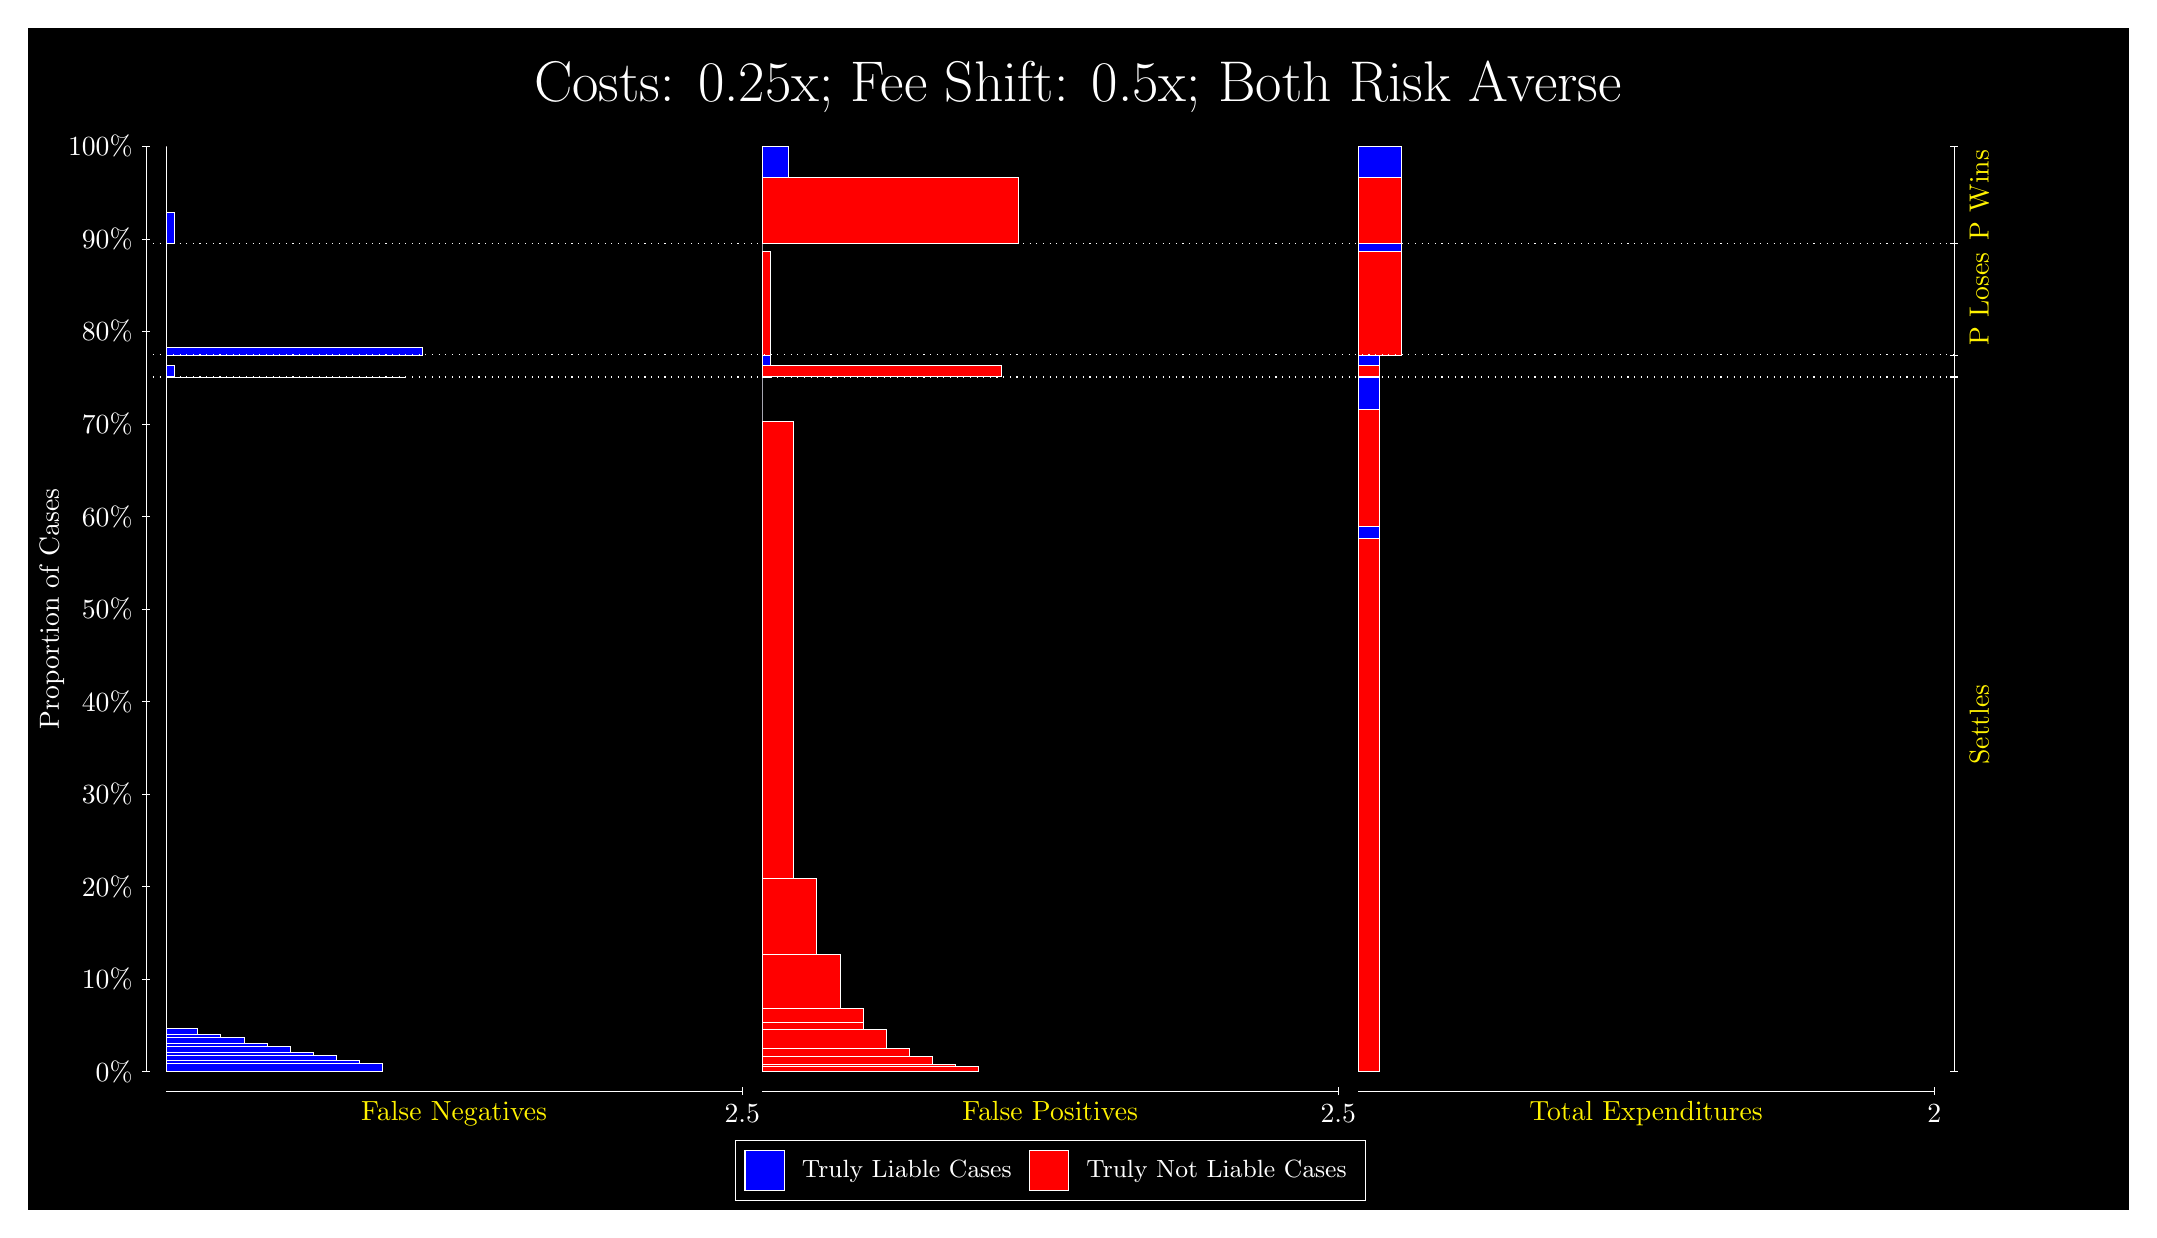
\begin{tikzpicture}
\draw[fill=black] (0,0) rectangle (26.667,15);
\draw[text=white] (0,13.5) rectangle (26.667,15) node[midway] {\huge Costs: 0.25x; Fee Shift: 0.5x; Both Risk Averse};
\draw[white, very thin] (1.5,1.75) -- (1.5,13.5);
\node[rotate=90, text=white, anchor=center] at (0.3, 7.625) {Proportion of Cases};
\draw[white, very thin] (1.45,1.75) -- (1.55,1.75);
\node[text=white, anchor=east] at (1.45, 1.75) {0\%};
\draw[white, very thin] (1.45,2.925) -- (1.55,2.925);
\node[text=white, anchor=east] at (1.45, 2.925) {10\%};
\draw[white, very thin] (1.45,4.1) -- (1.55,4.1);
\node[text=white, anchor=east] at (1.45, 4.1) {20\%};
\draw[white, very thin] (1.45,5.275) -- (1.55,5.275);
\node[text=white, anchor=east] at (1.45, 5.275) {30\%};
\draw[white, very thin] (1.45,6.45) -- (1.55,6.45);
\node[text=white, anchor=east] at (1.45, 6.45) {40\%};
\draw[white, very thin] (1.45,7.625) -- (1.55,7.625);
\node[text=white, anchor=east] at (1.45, 7.625) {50\%};
\draw[white, very thin] (1.45,8.8) -- (1.55,8.8);
\node[text=white, anchor=east] at (1.45, 8.8) {60\%};
\draw[white, very thin] (1.45,9.975) -- (1.55,9.975);
\node[text=white, anchor=east] at (1.45, 9.975) {70\%};
\draw[white, very thin] (1.45,11.15) -- (1.55,11.15);
\node[text=white, anchor=east] at (1.45, 11.15) {80\%};
\draw[white, very thin] (1.45,12.325) -- (1.55,12.325);
\node[text=white, anchor=east] at (1.45, 12.325) {90\%};
\draw[white, very thin] (1.45,13.5) -- (1.55,13.5);
\node[text=white, anchor=east] at (1.45, 13.5) {100\%};

\draw[white, very thin] (24.457,1.75) -- (24.457,13.5);
\draw[white, very thin] (24.407,1.75) -- (24.507,1.75);
\node[anchor=west] at (24.407, 1.75) {};
\draw[white, very thin] (24.407,10.567) -- (24.507,10.567);
\node[anchor=west] at (24.407, 10.567) {};
\draw[white, very thin] (24.407,10.582) -- (24.507,10.582);
\node[anchor=west] at (24.407, 10.582) {};
\draw[white, very thin] (24.407,10.851) -- (24.507,10.851);
\node[anchor=west] at (24.407, 10.851) {};
\draw[white, very thin] (24.407,12.263) -- (24.507,12.263);
\node[anchor=west] at (24.407, 12.263) {};
\draw[white, very thin] (24.407,13.5) -- (24.507,13.5);
\node[anchor=west] at (24.407, 13.5) {};

\draw[white, very thin, fill=blue] (1.75,1.75) rectangle (4.4946,1.86);
\draw[white, very thin, fill=blue] (1.75,1.86) rectangle (4.2018,1.8958);
\draw[white, very thin, fill=blue] (1.75,1.8958) rectangle (3.9091,1.9505);
\draw[white, very thin, fill=blue] (1.75,1.9505) rectangle (3.6163,1.992);
\draw[white, very thin, fill=blue] (1.75,1.992) rectangle (3.3236,2.0657);
\draw[white, very thin, fill=blue] (1.75,2.0657) rectangle (3.0308,2.1095);
\draw[white, very thin, fill=blue] (1.75,2.1095) rectangle (2.738,2.1835);
\draw[white, very thin, fill=blue] (1.75,2.1835) rectangle (2.4453,2.2208);
\draw[white, very thin, fill=blue] (1.75,2.2208) rectangle (2.1525,2.3056);
\draw[white, very thin, fill=red] (1.75,2.3056) rectangle (1.75,10.567);
\draw[white, very thin, fill=blue] (1.75,10.567) rectangle (4.7873,10.568);
\draw[white, very thin, fill=red] (1.75,10.568) rectangle (1.75,10.582);
\draw[white, very thin, fill=blue] (1.75,10.582) rectangle (1.8598,10.715);
\draw[white, very thin, fill=red] (1.75,10.715) rectangle (1.75,10.851);
\draw[white, very thin, fill=blue] (1.75,10.851) rectangle (5.0069,10.944);
\draw[white, very thin, fill=red] (1.75,10.944) rectangle (1.75,12.263);
\draw[white, very thin, fill=blue] (1.75,12.263) rectangle (1.8598,12.657);
\draw[white, very thin, fill=red] (1.75,12.657) rectangle (1.75,13.5);
\draw[white, very thin, fill=red] (9.3189,1.75) rectangle (12.063,1.8135);
\draw[white, very thin, fill=red] (9.3189,1.8135) rectangle (11.771,1.8462);
\draw[white, very thin, fill=red] (9.3189,1.8462) rectangle (11.478,1.9451);
\draw[white, very thin, fill=red] (9.3189,1.9451) rectangle (11.185,2.0423);
\draw[white, very thin, fill=red] (9.3189,2.0423) rectangle (10.892,2.2923);
\draw[white, very thin, fill=red] (9.3189,2.2923) rectangle (10.6,2.374);
\draw[white, very thin, fill=red] (9.3189,2.374) rectangle (10.6,2.5585);
\draw[white, very thin, fill=red] (9.3189,2.5585) rectangle (10.307,3.2371);
\draw[white, very thin, fill=red] (9.3189,3.2371) rectangle (10.014,4.2039);
\draw[white, very thin, fill=red] (9.3189,4.2039) rectangle (9.7214,10.012);
\draw[white, very thin, fill=blue] (9.3189,10.012) rectangle (9.3189,10.567);
\draw[white, very thin, fill=red] (9.3189,10.567) rectangle (9.4287,10.581);
\draw[white, very thin, fill=blue] (9.3189,10.581) rectangle (9.3189,10.582);
\draw[white, very thin, fill=red] (9.3189,10.582) rectangle (12.356,10.719);
\draw[white, very thin, fill=blue] (9.3189,10.719) rectangle (9.4287,10.851);
\draw[white, very thin, fill=red] (9.3189,10.851) rectangle (9.4287,12.171);
\draw[white, very thin, fill=blue] (9.3189,12.171) rectangle (9.3189,12.263);
\draw[white, very thin, fill=red] (9.3189,12.263) rectangle (12.576,13.106);
\draw[white, very thin, fill=blue] (9.3189,13.106) rectangle (9.6482,13.5);
\draw[white, very thin, fill=red] (16.888,1.75) rectangle (17.162,8.5247);
\draw[white, very thin, fill=blue] (16.888,8.5247) rectangle (17.162,8.6705);
\draw[white, very thin, fill=red] (16.888,8.6705) rectangle (17.162,10.158);
\draw[white, very thin, fill=blue] (16.888,10.158) rectangle (17.162,10.567);
\draw[white, very thin, fill=red] (16.888,10.567) rectangle (17.162,10.581);
\draw[white, very thin, fill=blue] (16.888,10.581) rectangle (17.162,10.582);
\draw[white, very thin, fill=red] (16.888,10.582) rectangle (17.162,10.719);
\draw[white, very thin, fill=blue] (16.888,10.719) rectangle (17.162,10.851);
\draw[white, very thin, fill=red] (16.888,10.851) rectangle (17.437,12.171);
\draw[white, very thin, fill=blue] (16.888,12.171) rectangle (17.437,12.263);
\draw[white, very thin, fill=red] (16.888,12.263) rectangle (17.437,13.106);
\draw[white, very thin, fill=blue] (16.888,13.106) rectangle (17.437,13.5);
\draw[white, dotted] (1.5,10.567) -- (24.457,10.567);
\draw[white, dotted] (1.5,10.582) -- (24.457,10.582);
\draw[white, dotted] (1.5,10.851) -- (24.457,10.851);
\draw[white, dotted] (1.5,12.263) -- (24.457,12.263);
\draw[white, very thin] (1.75,1.5) -- (9.0689,1.5);
\node[text=yellow, anchor=north] at (5.4094, 1.5) {False Negatives};
\draw[white, very thin] (9.0689,1.45) -- (9.0689,1.55);
\node[text=white, anchor=north] at (9.0689, 1.45) {2.5};

\draw[white, very thin] (9.3189,1.5) -- (16.638,1.5);
\node[text=yellow, anchor=north] at (12.978, 1.5) {False Positives};
\draw[white, very thin] (16.638,1.45) -- (16.638,1.55);
\node[text=white, anchor=north] at (16.638, 1.45) {2.5};

\draw[white, very thin] (16.888,1.5) -- (24.207,1.5);
\node[text=yellow, anchor=north] at (20.547, 1.5) {Total Expenditures};
\draw[white, very thin] (24.207,1.45) -- (24.207,1.55);
\node[text=white, anchor=north] at (24.207, 1.45) {2};

\node[text=yellow, centered, rotate=90] at (24.777, 6.1587) {Settles};


\node[text=yellow, centered, rotate=90] at (24.777, 11.557) {P Loses};
\node[text=yellow, centered, rotate=90] at (24.777, 12.882) {P Wins};

\draw (12.978300999999998,1.5) node[draw=none] (baseCoordinate) {};
\begin{scope}[align=center]
        \matrix[scale=0.5, draw=white, below=0.5cm of baseCoordinate, nodes={draw}, column sep=0.1cm]{
            \node[rectangle, draw, minimum width=0.5cm, minimum height=0.5cm, fill=blue] {}; &
            \node[draw=none, font=\small, text=white] (B) {Truly Liable Cases}; &
            \node[rectangle, draw, minimum width=0.5cm, minimum height=0.5cm, fill=red] {}; &
            \node[draw=none, font=\small, text=white] (B) {Truly Not Liable Cases}; \\
            };
\end{scope}

\end{tikzpicture}
\end{document}